\documentclass[10pt]{beamer}

%STANDARD PREAMBLE
%https://tex.stackexchange.com/questions/68821/is-it-possible-to-create-a-latex-preamble-header
%\usepackage{/Users/mwojno01/Repos/latex_preamble/beamer_preamble}
\usepackage{/Users/miw267/Repos/csci246_spring2025/slides/preambles/beamer_preamble_for_CSCI246}


%%%
% SPECIFIC TO THIS DOCUMENT 
%%%
\let\warning\relax
\usepackage{fourier} % has warning  and danger symbols. However, it makes the bottoms tuff bold. 

\renewcommand{\ELBO}{\texttt{ELBO}}
\renewcommand{\Q}{\mathcal{Q}}


%%%%
% DOCUMENT 
%%%
\title{03/26/2026: Diffusion Overview}
\author{Reference: \textit{Deep Learning (Sec 20.1-20.2)}}
\date{CSCI 546: Diffusion Models}

\begin{document}
\maketitle

%\begin{frame}{Table of contents}
%  \setbeamertemplate{section in toc}[sections numbered]
%  \tableofcontents[hideallsubsections]
%\end{frame}

\begin{frame}{Table of contents}
  \setbeamertemplate{section in toc}[sections numbered]
  \setbeamertemplate{subsection in toc}[subsections numbered]
  \tableofcontents
\end{frame}





\section{Course Logistics}



\begin{frame}
\begin{myredbox}[title=Announcements]

\begin{itemize}
	\item I have previous reading surveys to return. \pause 
	\item One reading survey will be dropped from your total score when computing your course grade.  This can help to cover absences for any reason, or just an off day. \pause 
	\item Please get back to me by \textbf{4pm today} on if/when  you want to retake the midterm.  \pause 
	\item If relevant, please check in with your lightning chat co-presenter to determine if you want to present together (preferred) or separately.  
\end{itemize}
\end{myredbox}
\end{frame}


\begin{frame}{Reading Survey}

\begin{enumerate}
	\item Describe the forward encoder of a diffusion model. (Sec 20.1)
	\item Describe the reverse decoder of a diffusion model. (Sec 20.2)
\end{enumerate}
	
\end{frame}


\section{Group Work Part I}

\begin{frame}{Random groups}
\begin{columns}
\begin{column}{0.33\textwidth}
Aubrey Williams: 8 \\ 
Austin Barton : 5 \\ 
Blake Sigmundstad: 6 \\ 
Diego Moylan: 7 \\ 
Dillon Shaffer: 7 \\ 
Ismoiljon Muzaffarov: 2 \\ 
Jacob Tanner: 1 \\\end{column}
\begin{column}{0.33\textwidth}
Josh Stoneback: 8 \\ 
Joshua Bowen: 6 \\ 
Joshua Culwell: 4 \\ 
Laura Banaszewski: 4 \\ 
Lina Hommel: 5 \\\end{column}
\begin{column}{0.33\textwidth}
Logan Racz: 1 \\ 
Matt Hall: 2 \\ 
Mike Kadoshnikov: 2 \\ 
Owen Cool: 3 \\ 
Racquel Bowen: 1 \\ 
Samuel Mocabee: 3 \\ 
Tatiana Kirillova: 3 \\\end{column}
\end{columns}	
\end{frame}



\begin{frame}{Group Exercises (Part I)}

\begin{enumerate}
	\item How do we know that if we define the forward process via the transition kernel $q(\+x_t \cond \+x_{t-1}) = \N(\+x_t; \sqrt{1-\beta_t} \+x_{t-1}, \beta_t \+I)$ that there is an equilibrium distribution, and moreover that the equilibrium distribution is $\pi = \N(\+0, \+I)$?
\end{enumerate} 

\vfill 
\pause 
\textit{Hint:} (Assuming that the kernel is aperiodic and $\pi$-irreducible), it suffices to verify detailed balance:

That is, we must show 
\[ \pi(y) q(x \cond y) \stackrel{?}{=} \pi(x) q(y \cond x) \] 

	
\end{frame}


%\begin{frame}{Good, Bad, Ugly, Beautiful}
%
%\textbf{Guidelines}
%Fill this out
%\begin{enumerate}
%	\item \textit{Good, Bad}: Technical content
%	\item \textit{Ugly, Beautiful}: Presentational styles
%\end{enumerate}
%
%\vfill 
%
%
%\textbf{Format}
%\begin{enumerate}
%	\item Small group discussion  \alert{at whiteboards}.  (Fill out your responses there.)
%	\item Class discussion 
%\end{enumerate}
%	
%\end{frame}




\section{Lightning Chat}

\begin{frame}[standout]
Lightning Chat
\end{frame}

\section{Mini-Lecture}

\begin{frame}{Forward Encoder}
\small 
\only<1-4>{
\begin{center} 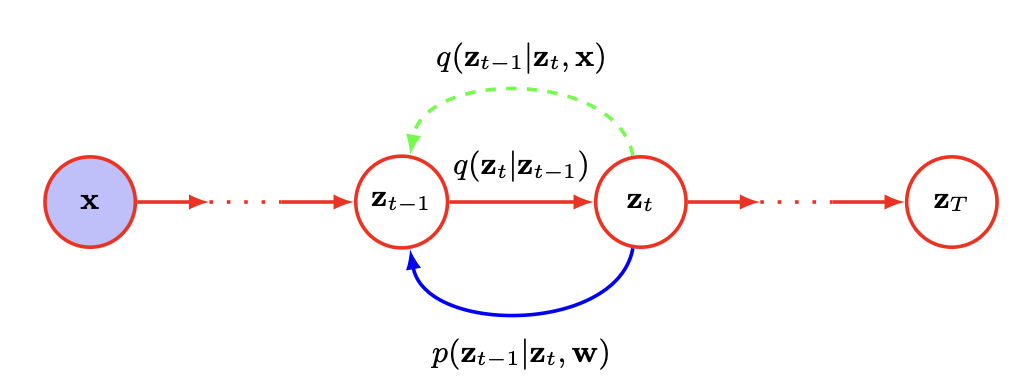
\includegraphics[width=.8\textwidth]{images/forward_process_bishop.png} 
\end{center}	
}
\only<5>{
\begin{center} 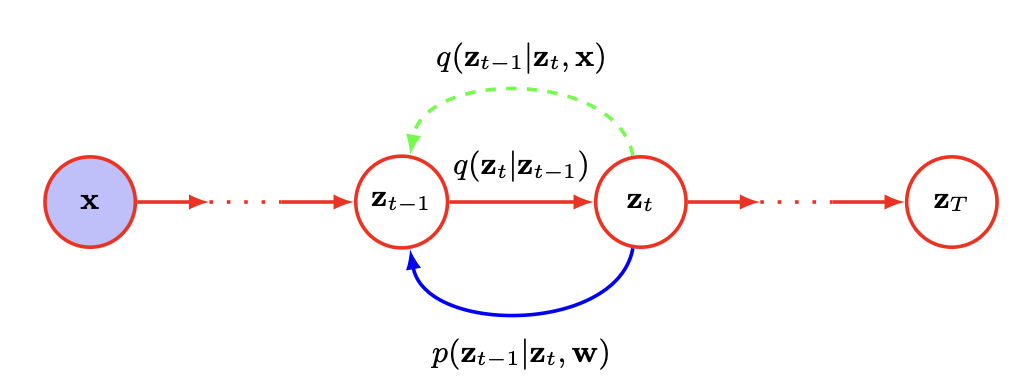
\includegraphics[width=.6\textwidth]{images/forward_process_bishop.png} 
\end{center}	
}

\uncover<2->{
The \textbf{forward transition kernel} is given by
%
\begin{align}
q(\+z_t \mid \+z_{t-1}) = \N\bigg( \sqrt{1-\beta_t}  \+z_{t-1} \, , \, \beta_t \+I\bigg)	
\label{eqn:forward_transition_kernel}
\end{align}
%
}%
\only<3>{
\hfill \hfill \scripttext{(for $t=1,\hdots,T$ if we define $\+z_0 \defeq \+x$)}
}%
%
\uncover<4->{As we will show (group exercise), by marginalizing over intermediate variables $\+z_1,\hdots, \+z_{t-1}$, we obtain the \textbf{diffusion kernel} as:
%
\begin{align}
 q(\+z_t \mid \+x) &= \N\bigg( \sqrt{\alpha_t}  \+x \, , \, (1-\alpha_t) \+I\bigg)	\label{eqn:diffusion_kernel} \\
 \text{where} \quad \alpha_t &\defeq \prod_{\tau=1}^t (1-\beta_t)  \nonumber 
\end{align}
}

\only<5->{\colorbox{yellow!30}{\textbf{Poll.}} What happens to \Eqref{eqn:diffusion_kernel} as $t$ increases?
}

\only<6->{\colorbox{green!30}{\textbf{Solution.}} 
\begin{columns}[c]
\column{0.5\textwidth}
\begin{itemize}
    \item the mean shrinks towards 0
    \item the covariance goes to identity matrix.
\end{itemize}


\column{0.5\textwidth}
\centering

\includegraphics[width=.4\linewidth]{images/bivariate_normal}
\end{columns}	
}


\end{frame}



\begin{frame}{Forward Encoder}

The \textbf{diffusion kernel} is obtained by marginalizing over $\+z_1,\hdots, \+z_{t-1}$:
%
\begin{align*}
 q(\+z_t \mid \+x) &= \N\bigg( \sqrt{\alpha_t}  \+x \, , \, (1-\alpha_t) \+I\bigg), \qquad \text{where} \quad \alpha_t \defeq \prod_{\tau=1}^t (1-\beta_t) 
\end{align*}
%
\pause 
\colorbox{yellow!30}{\textbf{Poll.}} Why do we care?
\pause 

\colorbox{green!30}{\textbf{Solution.}}

\begin{quotation}
We see that each intermediate distribution has a simple closed-form Gaussian expression from which we can directly sample, which will prove useful when training DDPMs as it allows efficient stochastic gradient descent [...] without having to run the whole chain.
\end{quotation}

\begin{center} 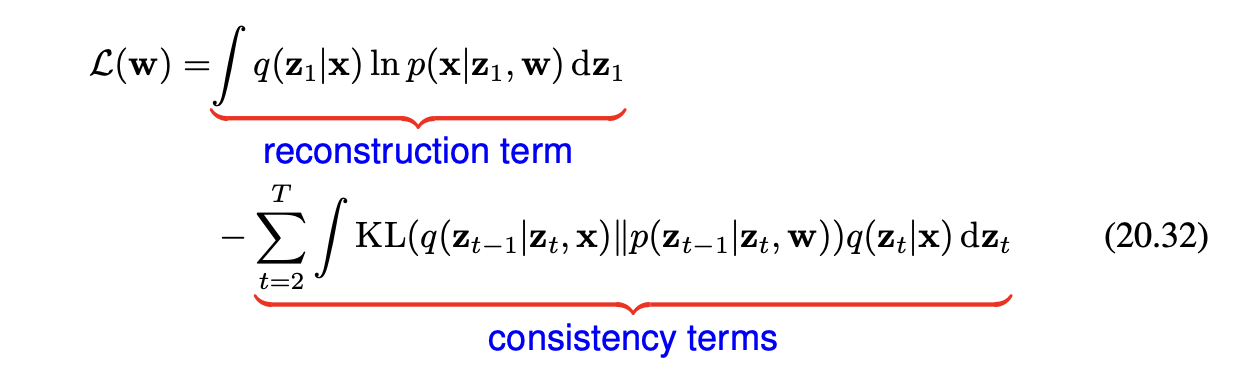
\includegraphics[width=.8\textwidth]{images/elbo} 
\end{center}


\end{frame}




\section{Group Work Part II}



\begin{frame}{Group Exercises (Part II)}


\colorbox{blue!30}{\textbf{Recall.}} The \textbf{forward transition kernel} is given by
%
\begin{align}
q(\+z_t \mid \+z_{t-1}) = \N\bigg( \sqrt{1-\beta_t}  \+z_{t-1} \, , \, \beta_t \+I\bigg)	
\label{eqn:forward_transition_kernel_2}
\end{align} %
The \textbf{diffusion kernel} is obtained by marginalizing over $\+z_1,\hdots, \+z_{t-1}$:
%
\begin{align}
 q(\+z_t \mid \+x) &= \N\bigg( \sqrt{\alpha_t}  \+x \, , \, (1-\alpha_t) \+I\bigg), \qquad \text{where} \quad \alpha_t \defeq \prod_{\tau=1}^t (1-\beta_t)  \label{eqn:diffusion_kernel} 
\end{align}
\vfill 

\colorbox{red!30}{\textbf{Exercise.}} Show that the marginal distribution of the forward process \Eqref{eqn:forward_transition_kernel_2} is given by \Eqref{eqn:diffusion_kernel}.

\begin{itemize}
	\item \textit{Hint:} Use induction. 
	\item \textit{Hint:} Use the fact that the sum of two independent Gaussian random variables is itself a Gaussian with additive means and covariances.
	\item \textit{Hint:} To use the above, rewrite \Eqref{eqn:forward_transition_kernel_2} as 
	\[ \+z_t = \sqrt{1-\beta_t}  \+z_{t-1} + \beta_t \+\epsilon_t, \qquad  \+\epsilon_t \sim \N(\+0,\+I)  \]
\end{itemize} 

\end{frame}


\section{Coding Up Diffusion}


\begin{frame}{Coding Up Diffusion}

\colorbox{green!30}{\textbf{Goal.}} The goal between now and next class: \alert{code up a simple diffusion model!} \pause 

\begin{enumerate}
\item \textit{Path 1}: Play with \bluelink{https://e-dorigatti.github.io/math/deep\%20learning/2023/06/25/diffusion.html}{Emilio's code}.  Some things you might do:
	\begin{itemize}
	\item Get it to work. 
	\item Try a different dataset (e. g. swiss roll, MNIST images)  
	\item Tweak it to run \underline{binomial} diffusion, apply to binary heartbeat data, as per Sohl-Dickstein et al (2015) Fig 2.
	\item Adjust codebase per ideas from the ML literature (e.g. add a diffusion schedule for the betas, such as a cosine schedule).  
	\end{itemize} \pause 
\item \textit{Path 2}: Rewrite Emilio's code using ideas presented in Bishop:
	\begin{itemize}
	\item Sec 20.2.3 Rewriting the ELBO 
	\item Sec 20.2.4 Predicting the noise.  
	\end{itemize} 
Do these changes improve results?
\end{enumerate}
\pause 
\colorbox{red!30}{\textbf{Format.}} Work in groups of two.  Tell me your partner before leaving.  Prepare a \textbf{5 min} \alert{(hard cap!)} presentation for next class showing us what you tried/learned. Note: This will probably just be 2-3 slides.  
\end{frame}

\end{document}

